% Copyright 2004 by Till Tantau <tantau@users.sourceforge.net>.
%
% In principle, this file can be redistributed and/or modified under
% the terms of the GNU Public License, version 2.
%
% However, this file is supposed to be a template to be modified
% for your own needs. For this reason, if you use this file as a
% template and not specifically distribute it as part of a another
% package/program, I grant the extra permission to freely copy and
% modify this file as you see fit and even to delete this copyright
% notice.

\documentclass{beamer}

\usepackage{tikz}
\usepackage[utf8]{inputenc}
\usetikzlibrary{automata, matrix,shapes.multipart,shapes.geometric,fit,scopes,positioning}

\definecolor{blue-base}{RGB}{42, 79, 110}
\definecolor{purple-custom}{RGB}{54, 51, 119}
\definecolor{orange-custom}{RGB}{227, 164, 79}
\definecolor{yellow-custom}{RGB}{170, 142, 57}

% There are many different themes available for Beamer. A comprehensive
% list with examples is given here:
% http://deic.uab.es/~iblanes/beamer_gallery/index_by_theme.html
% You can uncomment the themes below if you would like to use a different
% one:
%\usetheme{AnnArbor}
%\usetheme{Antibes}
%\usetheme{Bergen}
%\usetheme{Berkeley}
%\usetheme{Berlin}
%\usetheme{Boadilla}
%\usetheme{boxes}
%\usetheme{CambridgeUS}
%\usetheme{Copenhagen}
%\usetheme{Darmstadt}
%\usetheme{default}
%\usetheme{Frankfurt}
%\usetheme{Goettingen}
%\usetheme{Hannover}
%\usetheme{Ilmenau}
%\usetheme{JuanLesPins}
%\usetheme{Luebeck}
\usetheme{Madrid}
%\usetheme{Malmoe}
%\usetheme{Marburg}
%\usetheme{Montpellier}
%\usetheme{PaloAlto}
%\usetheme{Pittsburgh}
%\usetheme{Rochester}
%\usetheme{Singapore}
%\usetheme{Szeged}
%\usetheme{Warsaw}

\title{Mécanismes d'authentification}

% A subtitle is optional and this may be deleted
\subtitle{État de l'art}

\author{Matthieu~Nicolas}

\date{20/09/2016}

\subject{Theoretical Computer Science}

\AtBeginSection[]
{
  \begin{frame}<beamer>{Plan}
    \tableofcontents[currentsection]
  \end{frame}
}

\begin{document}

\begin{frame}
  \titlepage
\end{frame}

\begin{frame}{Plan}
  \tableofcontents
  % You might wish to add the option [pausesections]
\end{frame}

\section{Authentification locale}

\subsection{Principe}

\begin{frame}{Authentification locale}{Principe}
  \begin{center}
    \begin{itemize}
      \item Architecture la plus \emph{intuitive}
      \item L'application implémente son propre système d'authentification
    \end{itemize}
  \end{center}
\end{frame}

\subsection{Architecture}

\begin{frame}{Authentification locale}{Architecture}
  \begin{itemize}
    \item TODO
  \end{itemize}
\end{frame}

\subsection{Avantages vs Inconvénients}

\begin{frame}{Authentification locale}{Avantages vs Inconvénients}
  \begin{center}
    \begin{itemize}
      \item Avantages
      \begin{itemize}
        \item Solution relativement \emph{simple}
        \item Maîtrise de l'environnement
      \end{itemize}
      \pause
      \item Inconvénients
      \begin{itemize}
        \item \emph{Simple} de faire des erreurs
        \item Pas de distinction entre le service \emph{métier} et le service \emph{d'authentification}
        \item Un compte supplémentaire...
      \end{itemize}
    \end{itemize}
  \end{center}
\end{frame}

\subsection{Frameworks \& Librairies}

\begin{frame}{Authentification locale}{Frameworks \& Librairies}
  \begin{center}
    \begin{itemize}
    \item Available at \url{https://plm.telecomnancy.univ-lorraine.fr}
    \end{itemize}
  \end{center}
\end{frame}

\section{Authentification déléguée}

\subsection{Principe}

\begin{frame}{Authentification déléguée}{Principe}
  \begin{center}
    \begin{itemize}
      \item Sépare le rôle des composants
      \begin{itemize}
        \item \textbf{Fournisseur d'identité (Identity Provider)}
        \item \textbf{Fournisseur de service (Service Provider)}
      \end{itemize}
      \item Pour pouvoir utiliser le service, un utilisateur doit déjà fournir une preuve de son identité
      \item TODO
    \end{itemize}
  \end{center}
\end{frame}

\subsection{Architecture}

\begin{frame}{Architecture}
  \begin{center}
    \begin{itemize}
    \item Available at \url{https://plm.telecomnancy.univ-lorraine.fr}
    \end{itemize}
  \end{center}
\end{frame}

\subsection{Différences entre OpenID \& OAuth}

\begin{frame}{OpenID}
  \begin{center}
    \begin{itemize}
      \item Protocole d'\emph{authentification}
      \item TODO
    \end{itemize}
  \end{center}
\end{frame}

\begin{frame}{OAuth}
  \begin{center}
    \begin{itemize}
      \item Protocole d'\emph{autorisation}
      \item Ne parle pas de fournisseur d'identité, mais de \textbf{serveur de ressources (Resource server)}
      \item Permet à un utilisateur (\textbf{Resource owner}) de donner un accès à une ressource à une application tierce
      \item[~]
      \item Mais utilisé de façon détourné pour faire de la \emph{pseudo-authentification}
    \end{itemize}
  \end{center}
\end{frame}

\begin{frame}{Différences entre OpenID \& OAuth}
  \begin{center}
    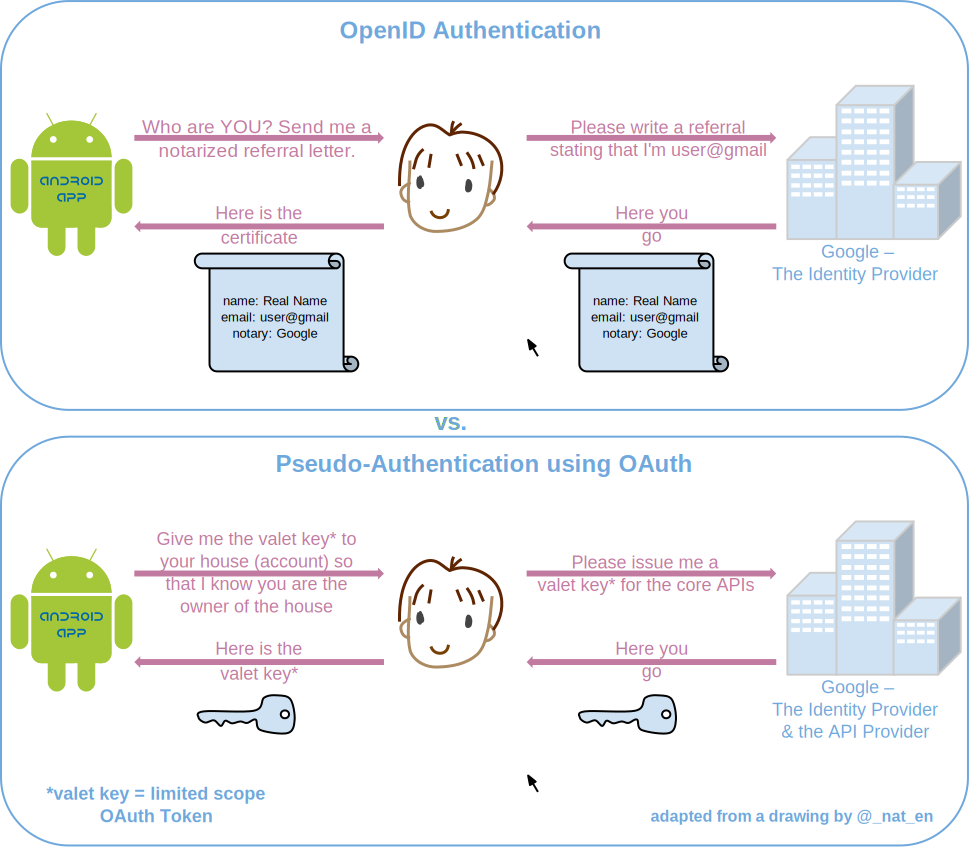
\includegraphics[width=0.75\textwidth]{img/OpenIDvsPseudo-AuthenticationusingOAuth}
  \end{center}
\end{frame}

\subsection{OpenID Connect}

\begin{frame}{OpenID Connect}
  \begin{center}
    \begin{itemize}
    \item Available at \url{https://plm.telecomnancy.univ-lorraine.fr}
    \end{itemize}
  \end{center}
\end{frame}

\subsection{Avantages vs Inconvénients}

\begin{frame}{Authentification déléguée}{Avantages vs Inconvénients}
  \begin{center}
    \begin{itemize}
      \item Avantages
      \begin{itemize}
        \item Interopérabilité
        \item Flexibilité
        \item Scalabilité
        \item SSO
        \item Pas besoin de partager les credentials
      \end{itemize}
      \item Inconvénients
      \begin{itemize}
        \item Plus \emph{compliqué} à bien implémenter
        \item Dépendant de services tiers
        \item Compte tiers compromis $\rightarrow$ Service compromis
      \end{itemize}
    \end{itemize}
  \end{center}
\end{frame}

\subsection{Frameworks \& Librairies}

\begin{frame}{Authentification déléguée}{Frameworks \& Librairies}
  \begin{center}
    \begin{itemize}
    \item Available at \url{https://plm.telecomnancy.univ-lorraine.fr}
    \end{itemize}
  \end{center}
\end{frame}

\section*{Thanks}

\begin{frame}{Questions}
  \begin{center}
    Merci pour votre attention, avez-vous des questions?
  \end{center}
\end{frame}

\end{document}
